\PassOptionsToPackage{quiet}{fontspec}
\documentclass[12pt,a4paper,UTF8]{article}
\usepackage{thesis} % 格式控制
\usepackage{indentfirst}
\usepackage{float}
\setlength{\parindent}{2em} % 控制首行缩进  
\addtolength{\parskip}{3pt} % 控制段落距离  
\onehalfspacing % 1.5倍行距  
\graphicspath{{./figures/}} % 指定图片所在文件夹  


\classname{Signal and System}  % 设置课程名称
\makepagestyle{}{\printclassname ~Experiment Report}
\begin{document}
\maketitlepage{Lab03}{西2-310}{Zhixuan Zheng}{3230103913}{\today}{Xiaoming Chen} % Cover page

\maketoc    %目录页

\section{Problem1}
\subsection{Problem}
\begin{figure}[H]
  \centering
  \begin{minipage}[b]{0.5\linewidth}
      \centering
      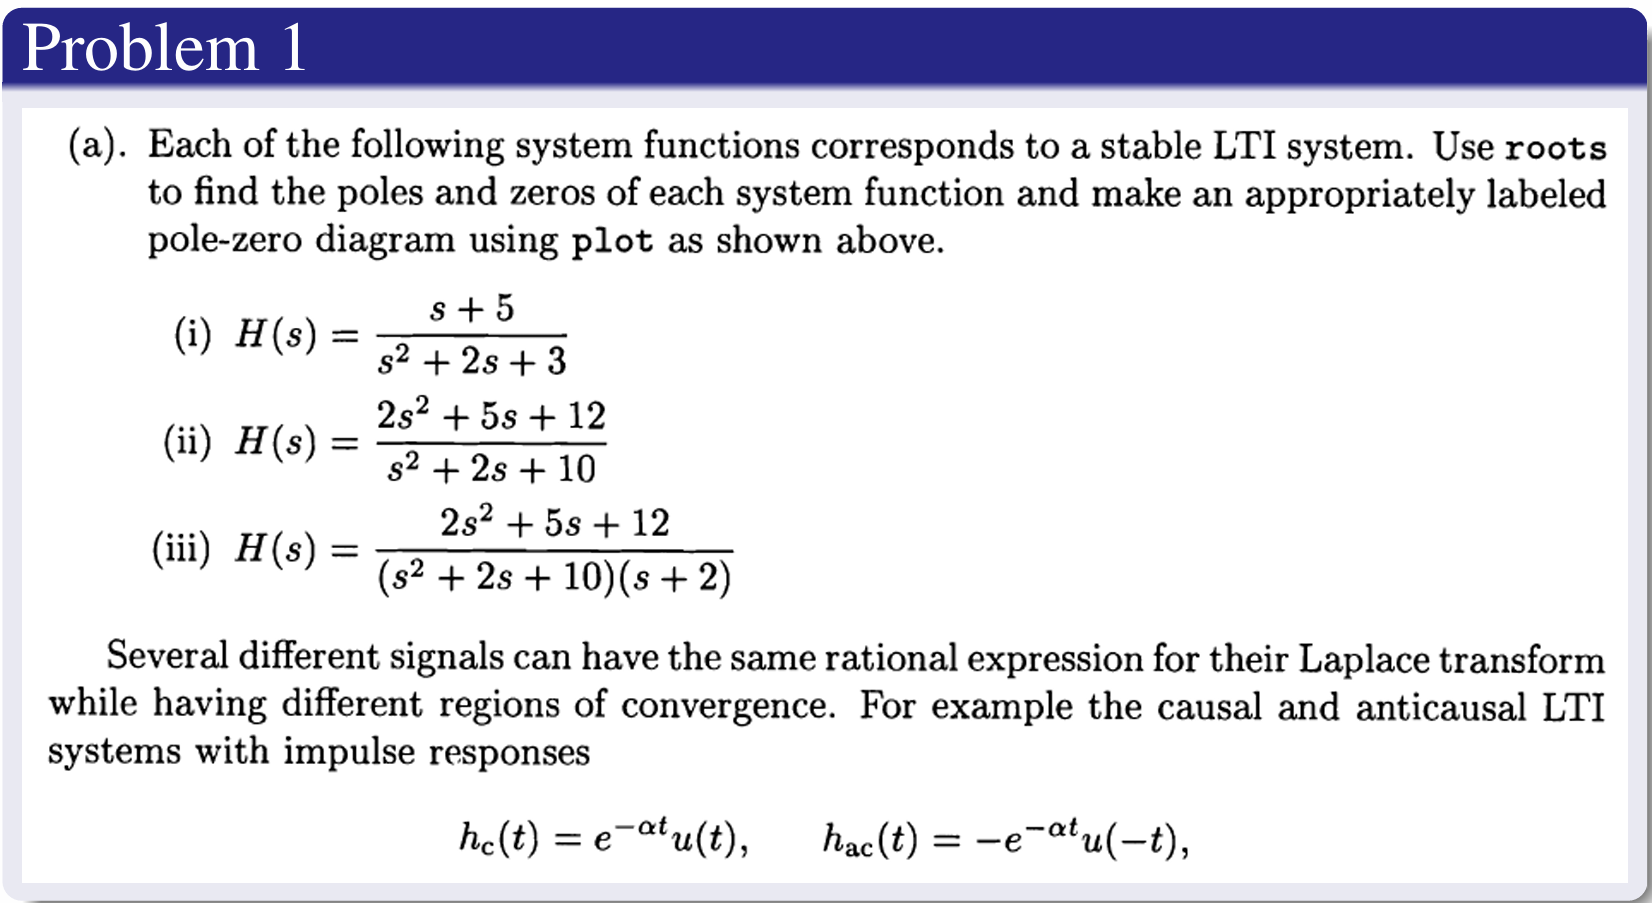
\includegraphics[width=0.9\textwidth]{figures/p11.png}
      \caption{Problem1}
  \end{minipage}%
  \begin{minipage}[b]{0.5\linewidth}
      \centering
      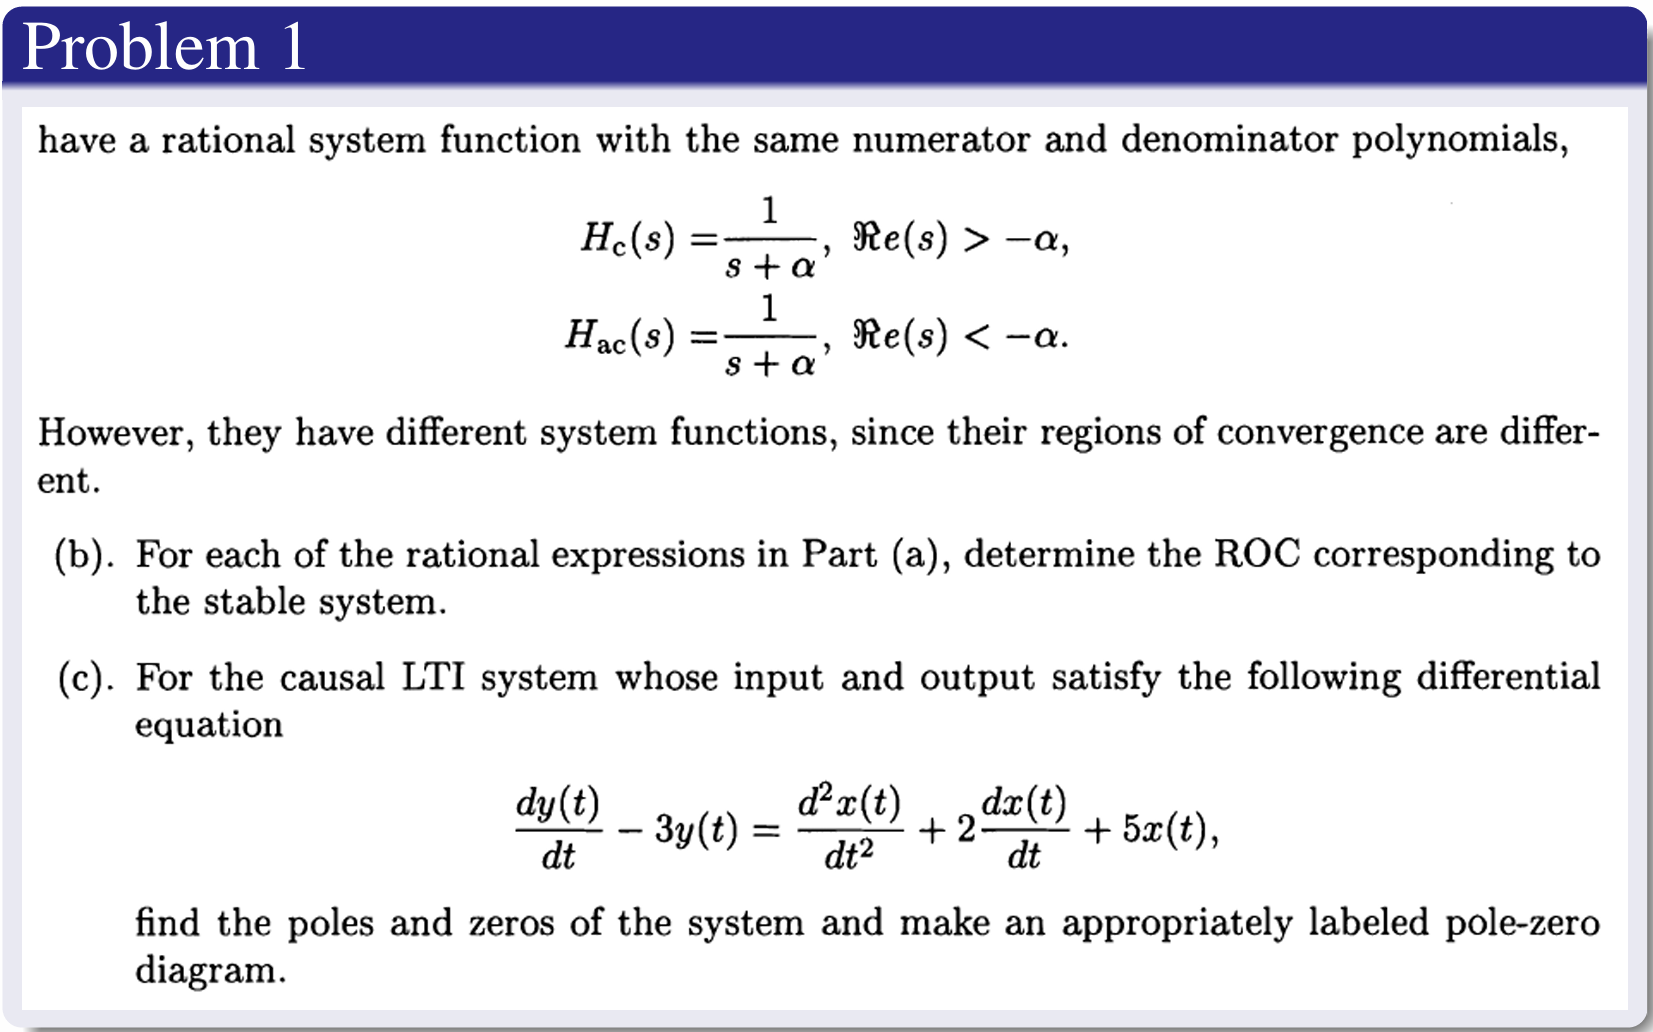
\includegraphics[width=0.9\textwidth]{figures/p12.png}
      \caption{Problem1}
  \end{minipage}
\end{figure}
\subsection{Answer}
\subsubsection{Answer(a)}

\begin{figure}[H]
  \centering
  \begin{minipage}[b]{0.33\linewidth}
      \centering
      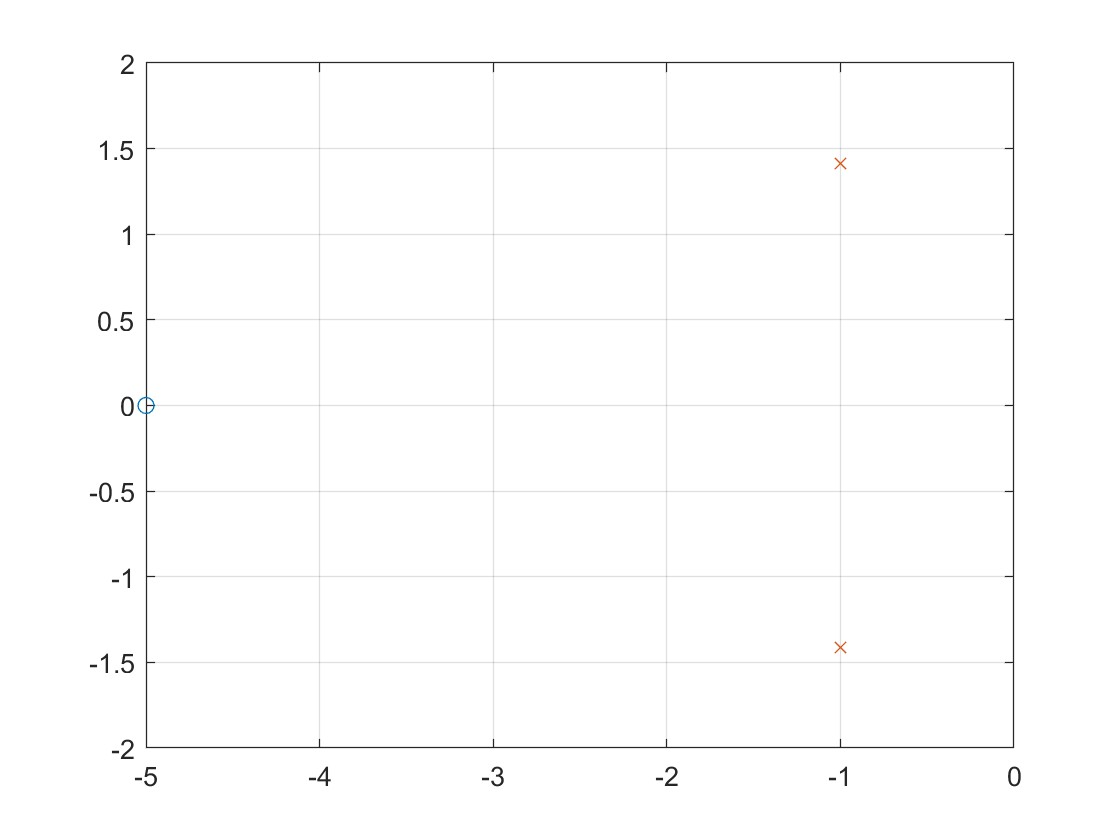
\includegraphics[width=0.9\textwidth]{figures/p1a1.jpg}
      \caption{Answer1a (i)}
  \end{minipage}%
  \begin{minipage}[b]{0.33\linewidth}
      \centering
      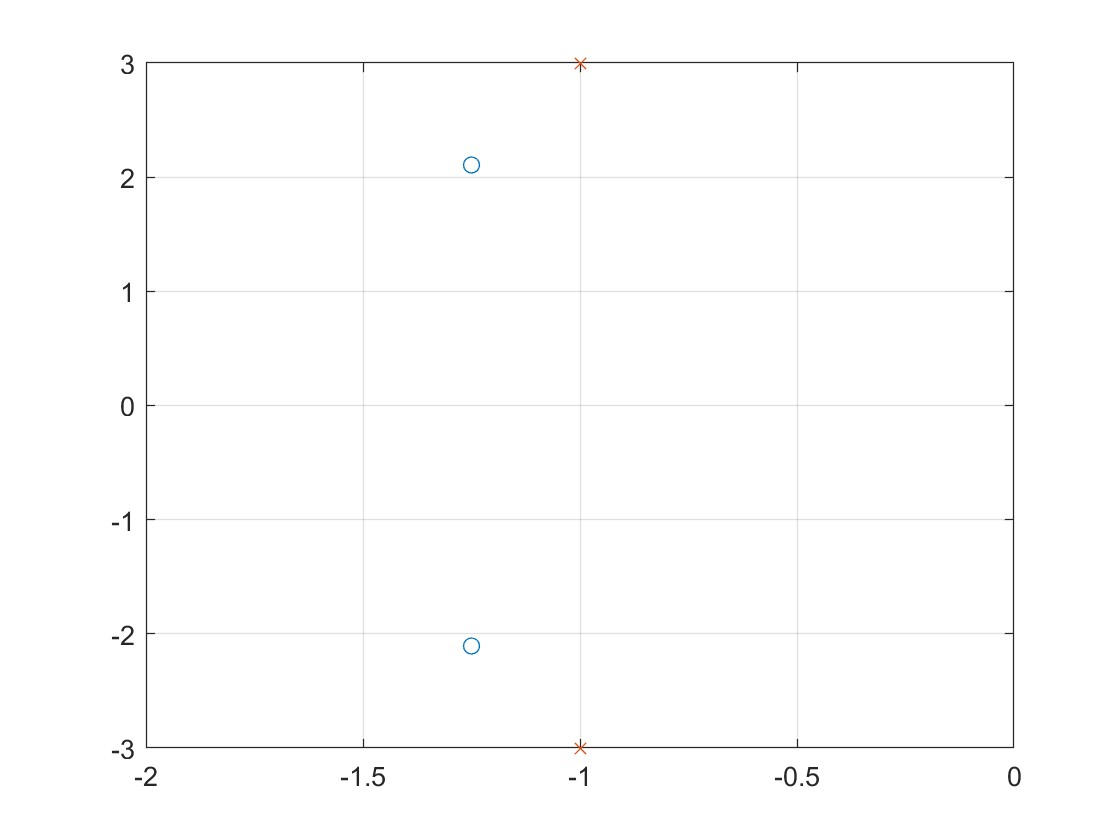
\includegraphics[width=0.9\textwidth]{figures/p1a2.jpg}
      \caption{Answer1a (ii)}
  \end{minipage}%
  \begin{minipage}[b]{0.33\linewidth}
      \centering
      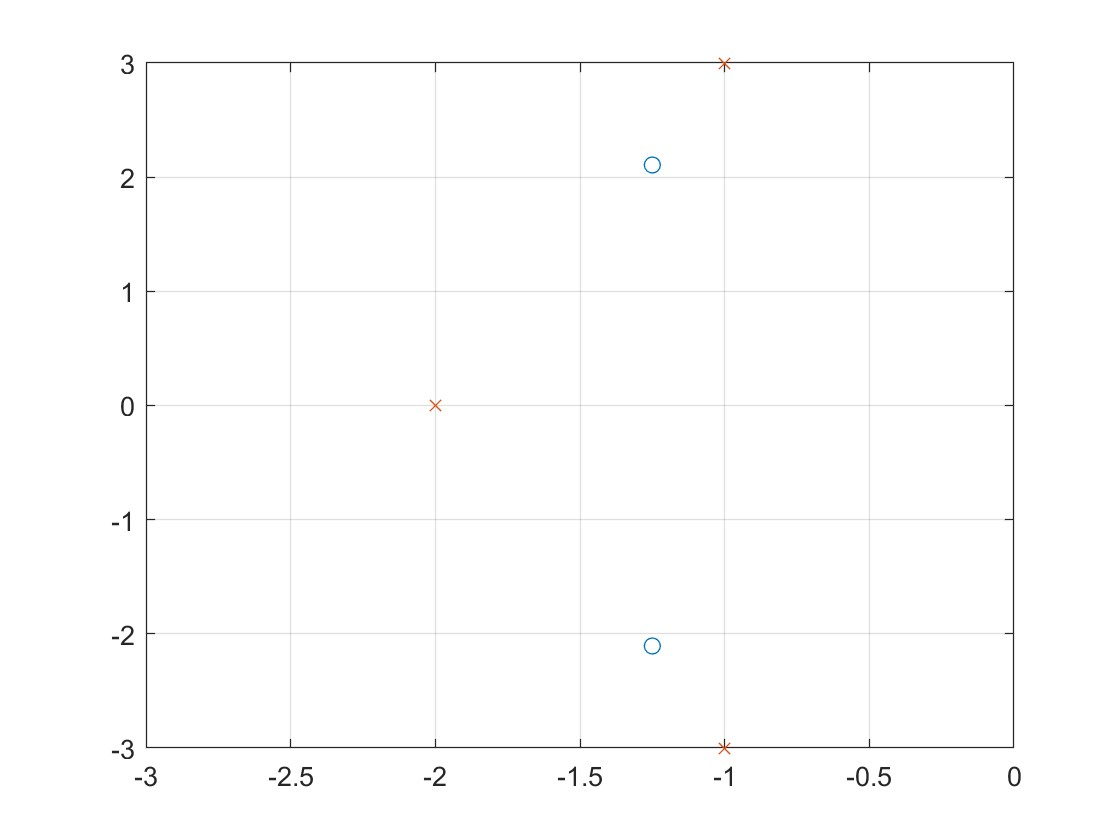
\includegraphics[width=0.9\textwidth]{figures/p1a3.jpg}
      \caption{Answer1a (iii)}
  \end{minipage}
\end{figure}

\subsubsection{Answer(b)}
(i)$ROC:Re(s)>-1$

(ii)$ROC:Re(s)>-1$

(iii)$ROC:Re(s)>-1$
\subsubsection{Answer(c)}

\begin{figure}[H]
  \centering
  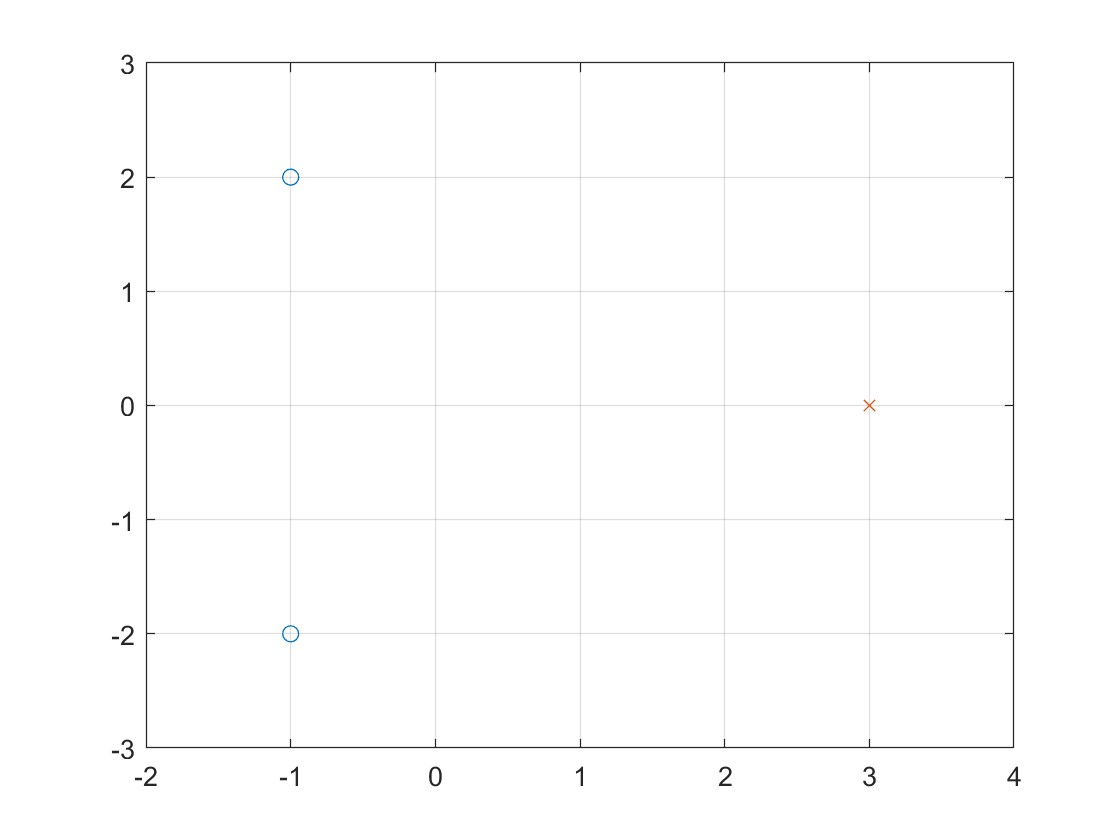
\includegraphics[width=0.5\linewidth]{figures/p1c.jpg} % 数字表示放缩比例
  \caption{Answer1c} % 图片标题
  \label{Prob1c} % 图片tag，用于交叉引用
\end{figure}

\clearpage
\section{Problem2}
\subsection{Problem}
\begin{figure}[H]
  \centering
  \begin{minipage}[b]{0.5\linewidth}
      \centering
      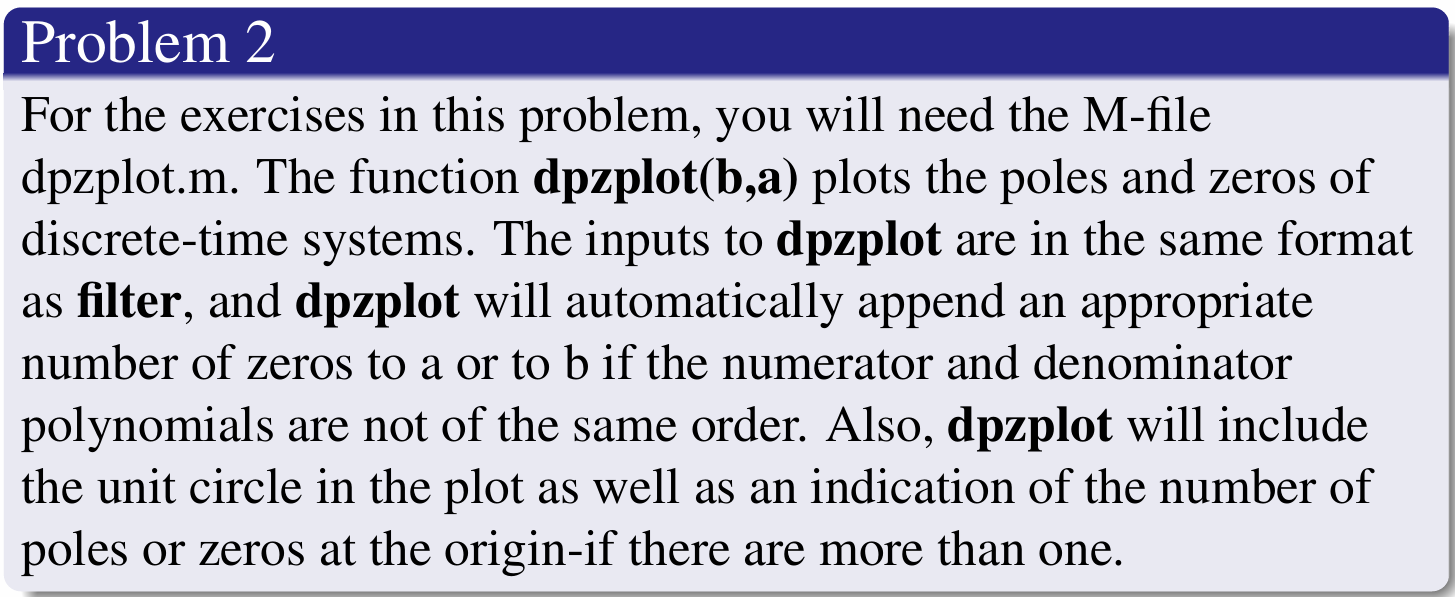
\includegraphics[width=0.9\textwidth]{figures/p21.png}
      \caption{Problem2}
  \end{minipage}%
  \begin{minipage}[b]{0.5\linewidth}
      \centering
      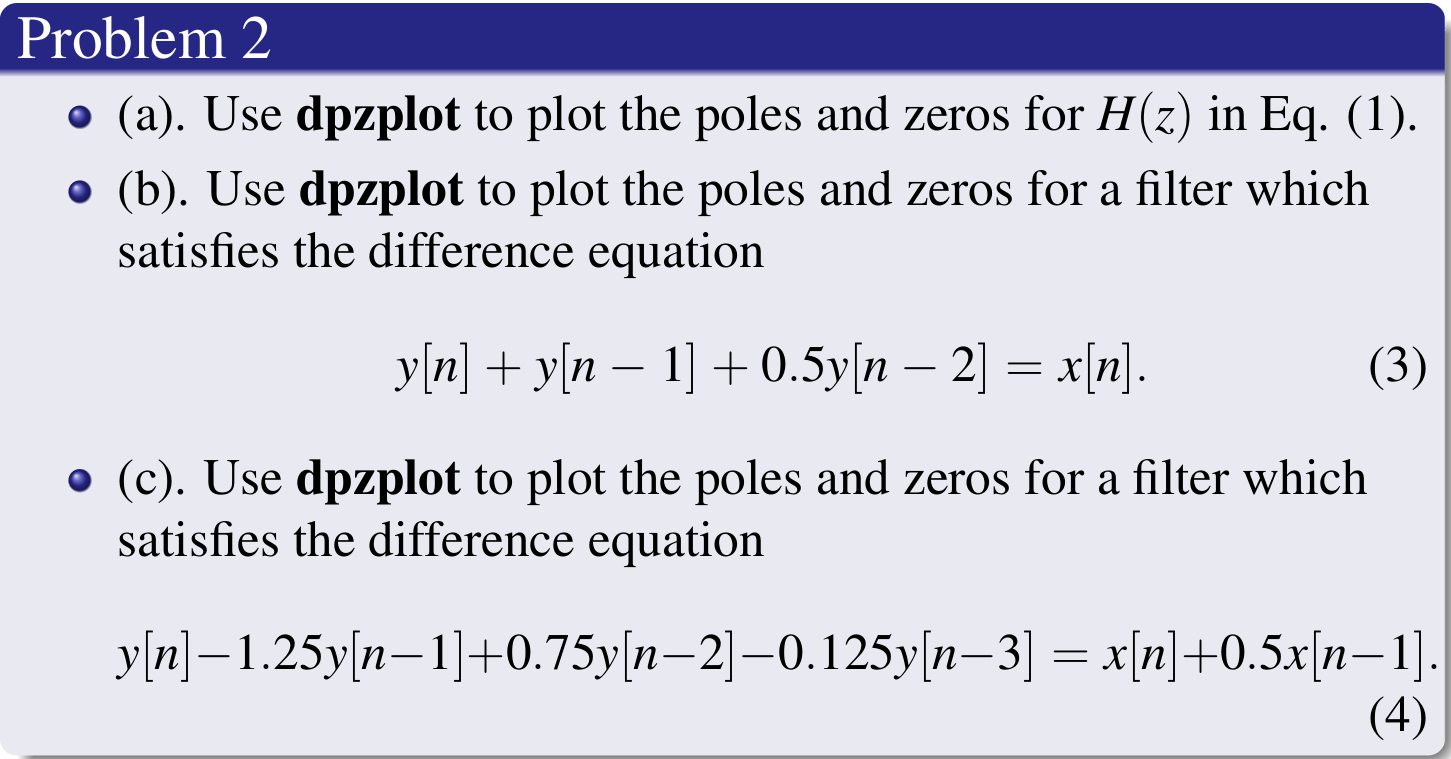
\includegraphics[width=0.9\textwidth]{figures/p22.png}
      \caption{Problem2}
  \end{minipage}
\end{figure}

\subsection{Answer}
\begin{figure}[H]
  \centering
  \begin{minipage}[b]{0.33\linewidth}
      \centering
      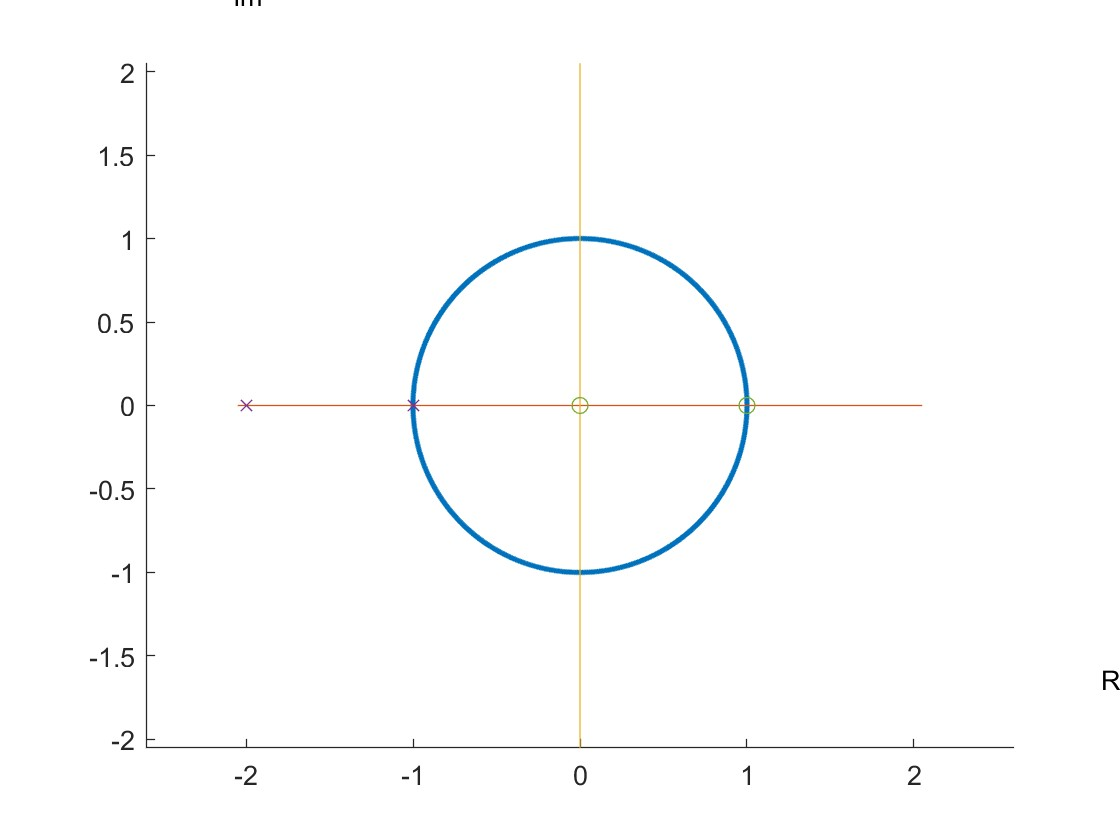
\includegraphics[width=0.9\textwidth]{figures/p2a.jpg}
      \caption{Answer2a}
  \end{minipage}%
  \begin{minipage}[b]{0.33\linewidth}
      \centering
      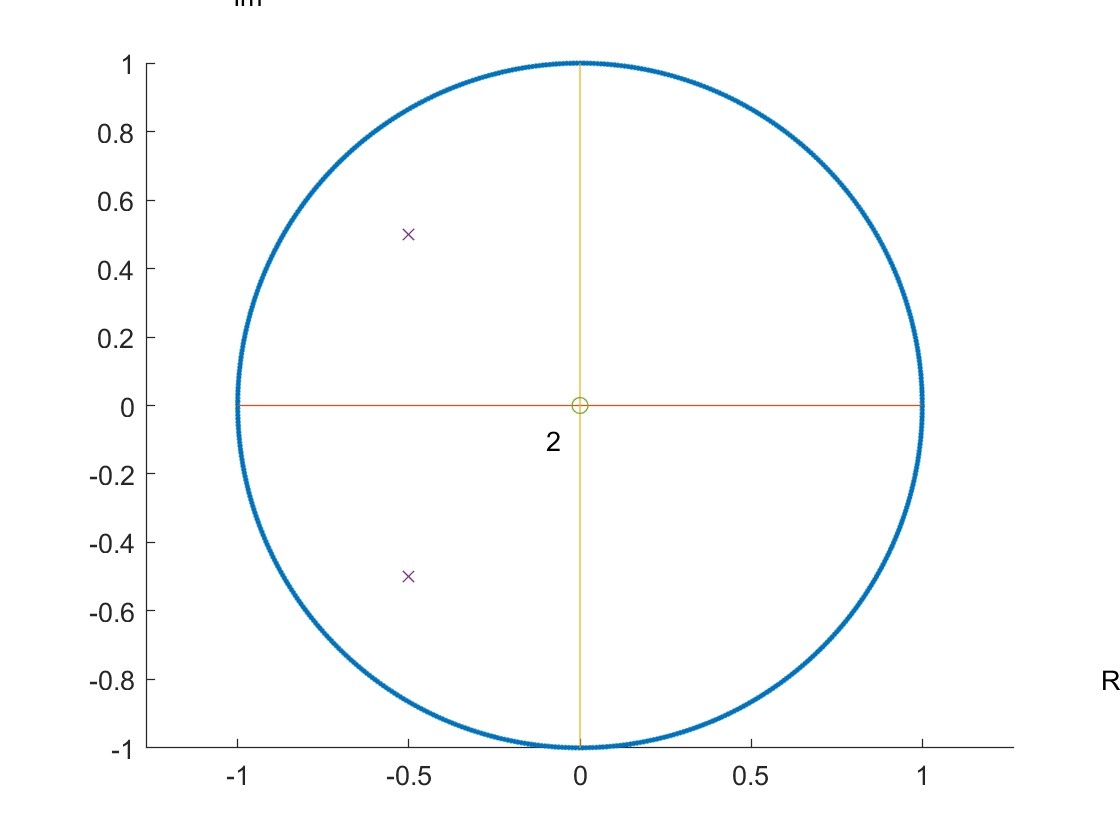
\includegraphics[width=0.9\textwidth]{figures/p2b.jpg}
      \caption{Answer2b}
  \end{minipage}%
  \begin{minipage}[b]{0.33\linewidth}
      \centering
      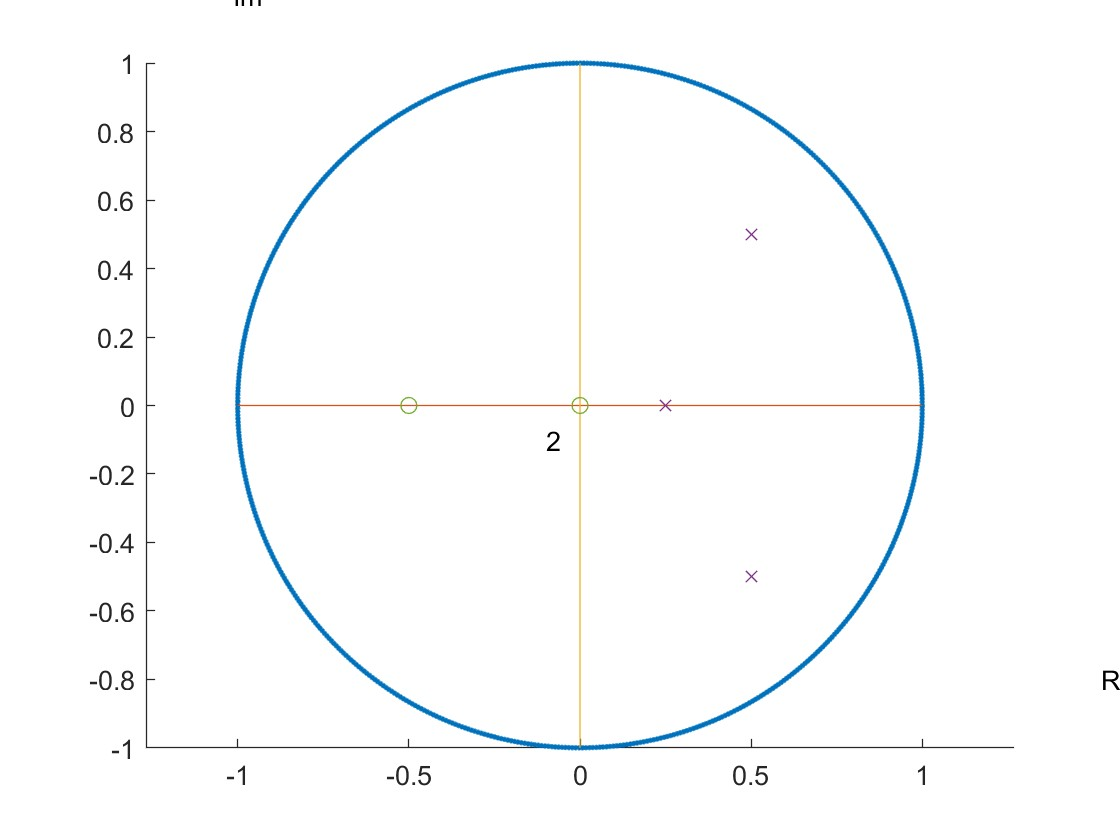
\includegraphics[width=0.9\textwidth]{figures/p2c.jpg}
      \caption{Answer2c}
  \end{minipage}
\end{figure}

\clearpage

\section{Problem3 a-g}
\subsection{Problem}
\begin{figure}[H]
  \centering
  \begin{minipage}[b]{0.5\linewidth}
      \centering
      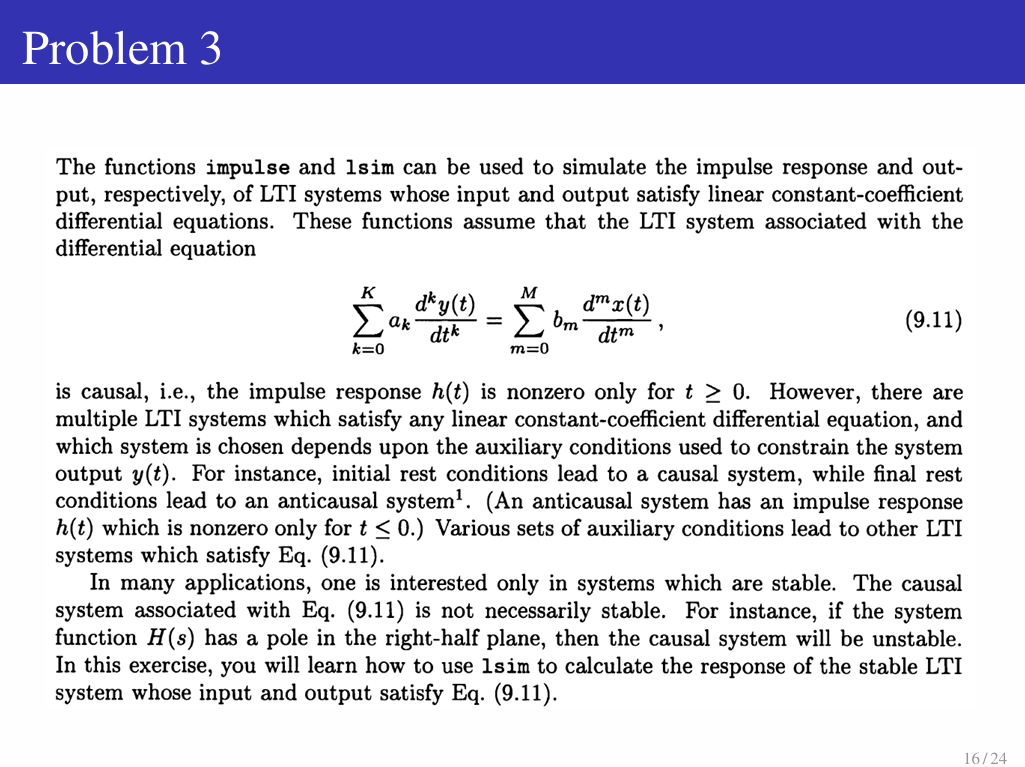
\includegraphics[width=0.9\textwidth]{figures/p31.png}
      \caption{Problem3}
  \end{minipage}%
  \begin{minipage}[b]{0.5\linewidth}
      \centering
      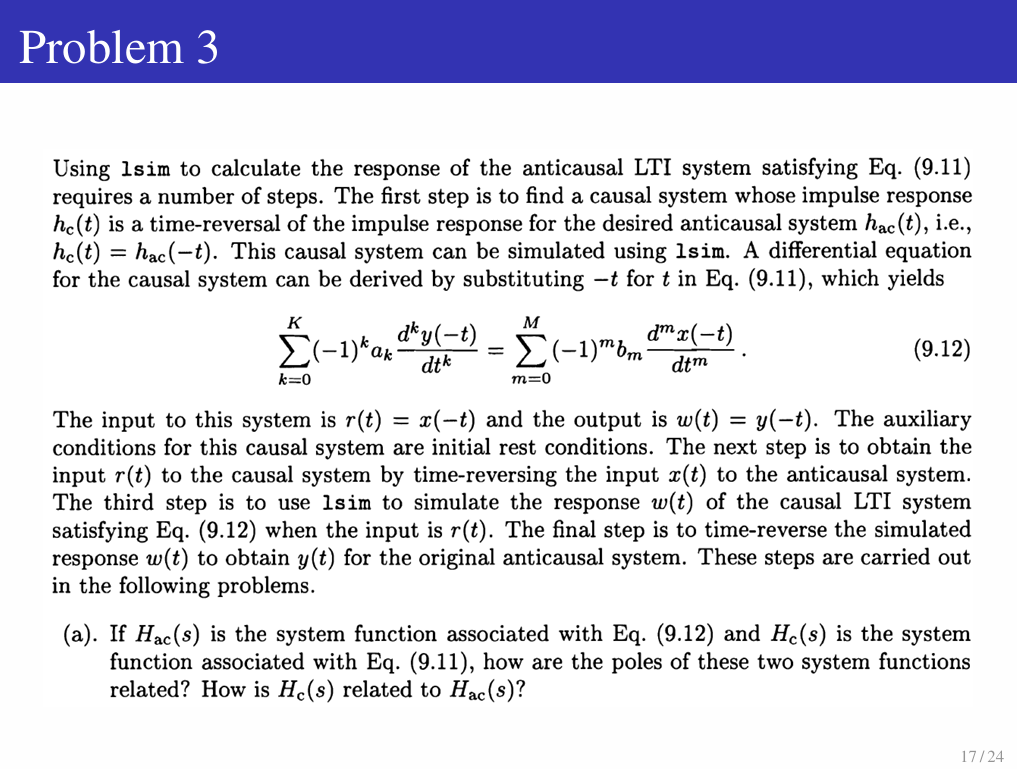
\includegraphics[width=0.9\textwidth]{figures/p32.png}
      \caption{Problem3}
  \end{minipage}
\end{figure}

\begin{figure}[H]
  \centering
  \begin{minipage}[b]{0.5\linewidth}
      \centering
      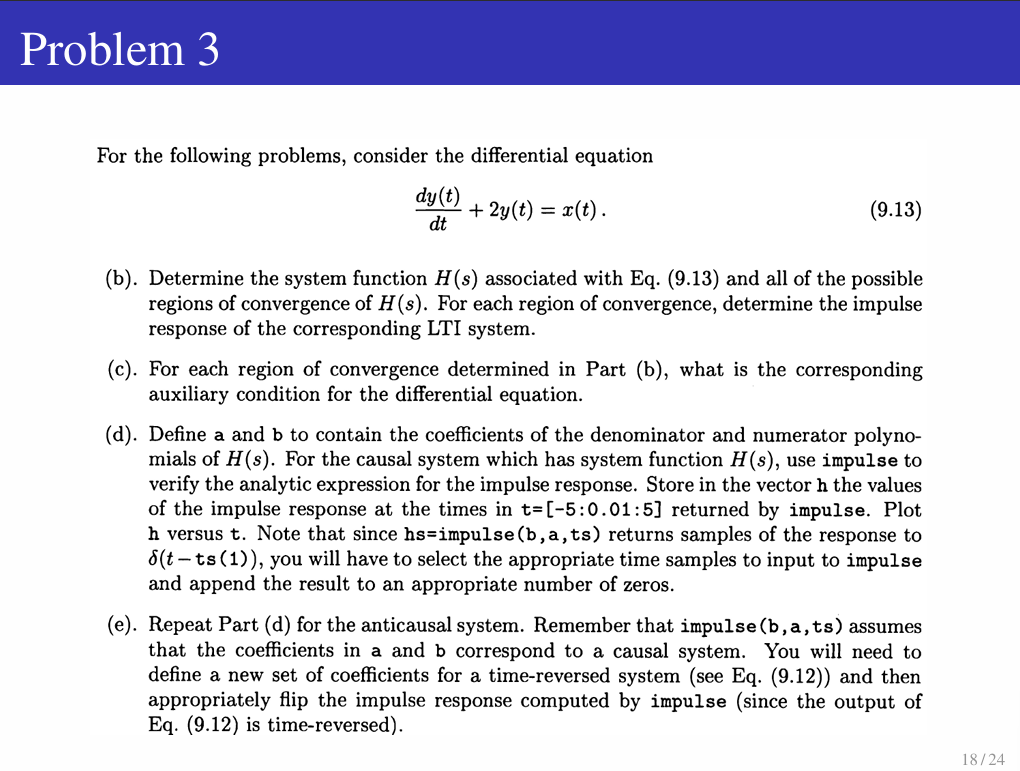
\includegraphics[width=0.9\textwidth]{figures/p33.png}
      \caption{Problem3}
  \end{minipage}%
  \begin{minipage}[b]{0.5\linewidth}
      \centering
      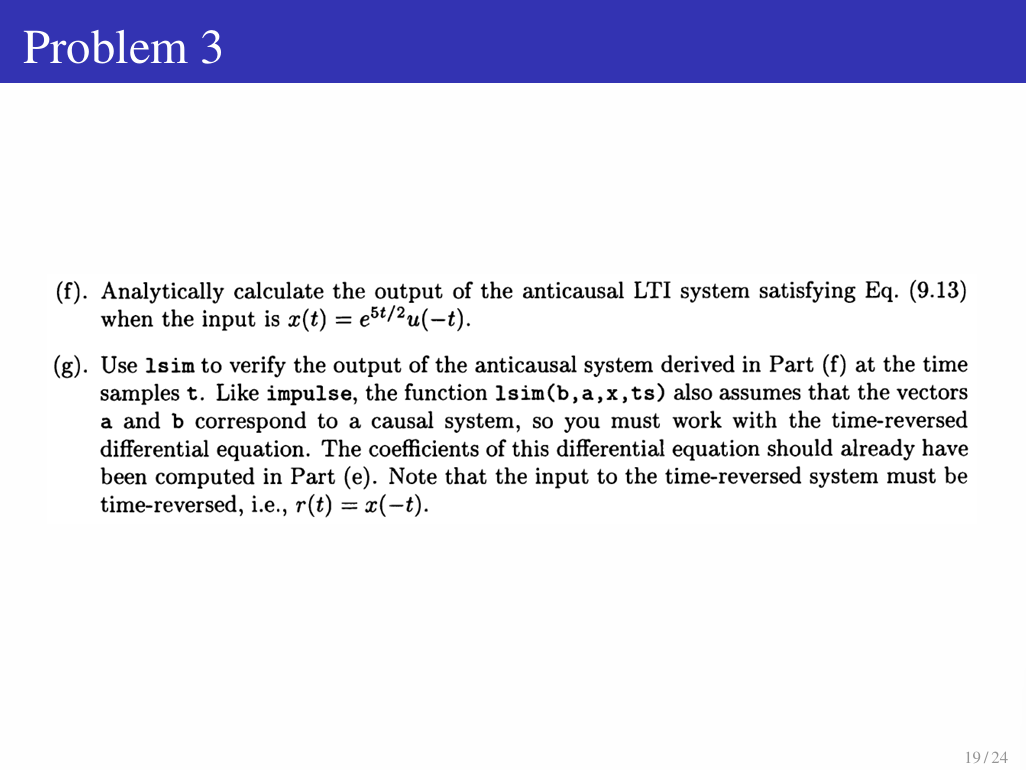
\includegraphics[width=0.9\textwidth]{figures/p34.png}
      \caption{Problem3}
  \end{minipage}
\end{figure}

\subsection{Answer}
\subsubsection{Answer a}
if $s_0$ the pole of $H_c(s)$,then
 $−s_0$ is the pole of $H_{ac}(s)$

$$H_{ac}(s)=H_c(-s)$$
\subsubsection{Answer b}
$$H(s) = \frac{Y(s)}{X(s)} = \frac{1}{s + 2}$$
$$\text{ROC: Re}\{s\} > -2 \ h(t) = e^{-2t}u(t) $$
$$\text{ROC: Re}\{s\} < -2 \ h(t) = -e^{-2t}u(-t)$$
\subsubsection{Answer c}
$\text{ROC: Re}\{s\} > -2$ initial rest conditions

$\text{ROC: Re}\{s\} < -2$ final rest conditions
\subsubsection{Answer d,e}
\begin{figure}[H]
  \centering
  \begin{minipage}[b]{0.5\linewidth}
      \centering
      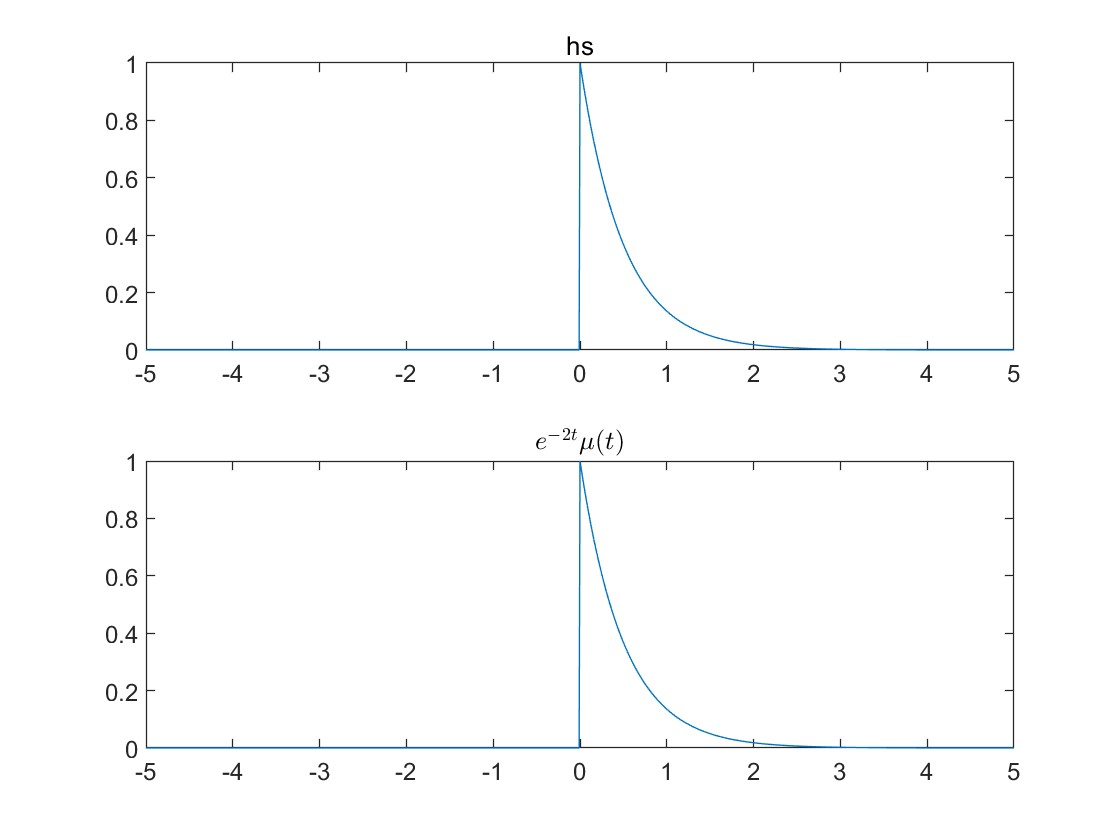
\includegraphics[width=0.9\textwidth]{figures/p3d.jpg}
      \caption{Answer3d}
  \end{minipage}%
  \begin{minipage}[b]{0.5\linewidth}
      \centering
      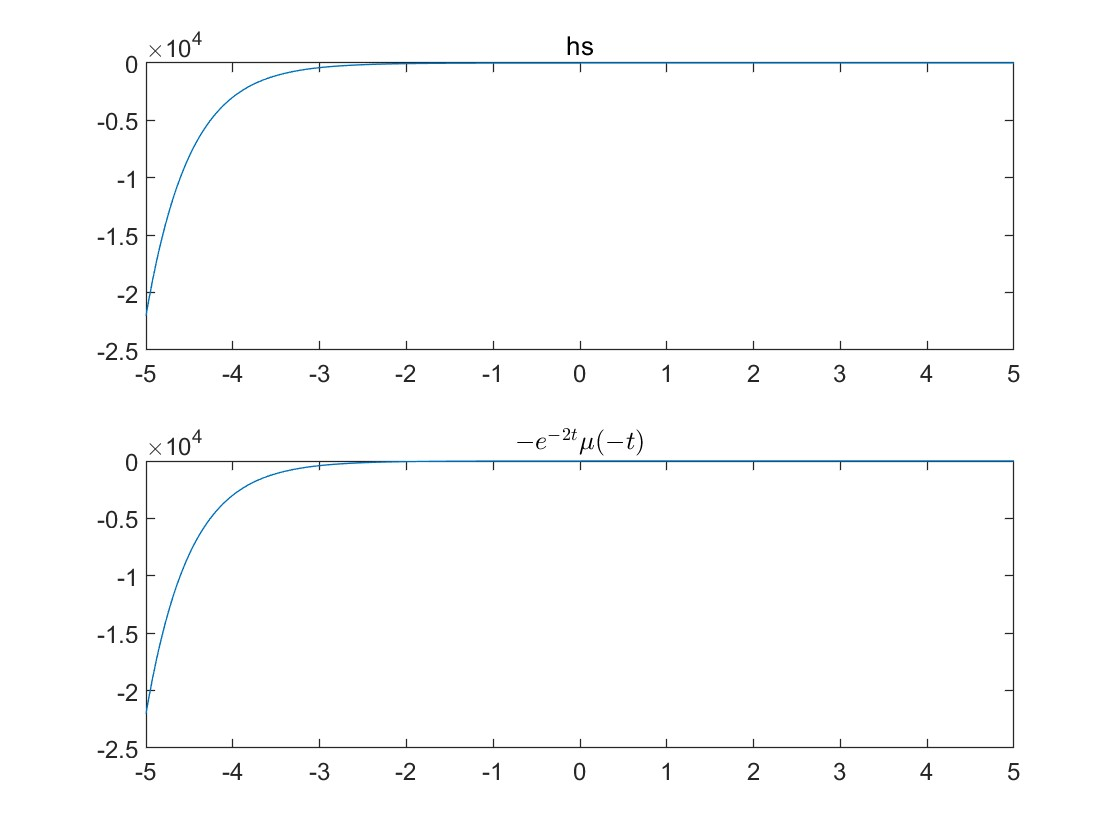
\includegraphics[width=0.9\textwidth]{figures/p3e.jpg}
      \caption{Answer3e}
  \end{minipage}
\end{figure}
\subsubsection{Answer f,g}
\[
X(s) = -\frac{1}{s - 2.5}
\]

\[
Y(s) = H(s) X(s) = -\frac{1}{(s + 2)(s - 2.5)}
\]

$$ \Rightarrow y=(\frac{2}{9} \cdot e^{\frac{5}{2}t}  - \frac{2}{9} \cdot e^{-2t}) \cdot u(-t) $$
\begin{figure}[H]
  \centering
  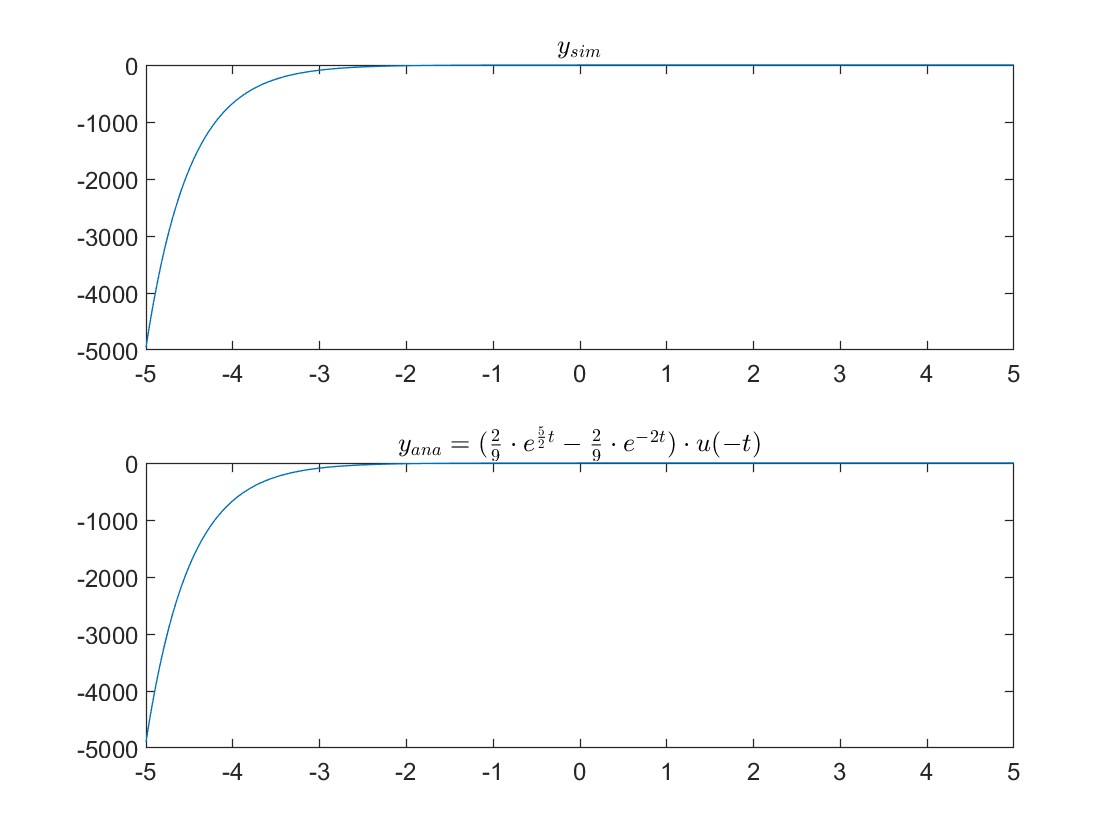
\includegraphics[width=0.5\linewidth]{figures/p3g.jpg} % 数字表示放缩比例
  \caption{Answer3g} % 图片标题
  \label{Prob1c} % 图片tag，用于交叉引用
\end{figure}

\clearpage

\section{Problem3 h-p}
\subsection{Problem}

\begin{figure}[H]
  \centering
  \begin{minipage}[b]{0.33\linewidth}
      \centering
      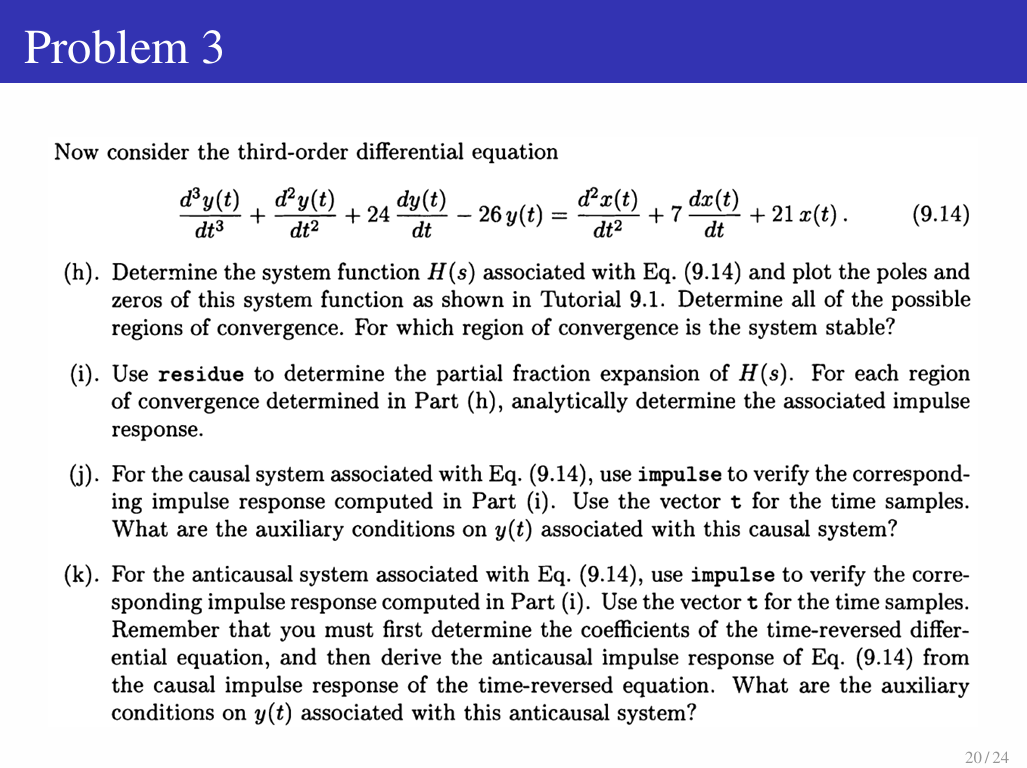
\includegraphics[width=0.9\textwidth]{figures/p35.png}
      \caption{Problem3}
  \end{minipage}%
  \begin{minipage}[b]{0.33\linewidth}
      \centering
      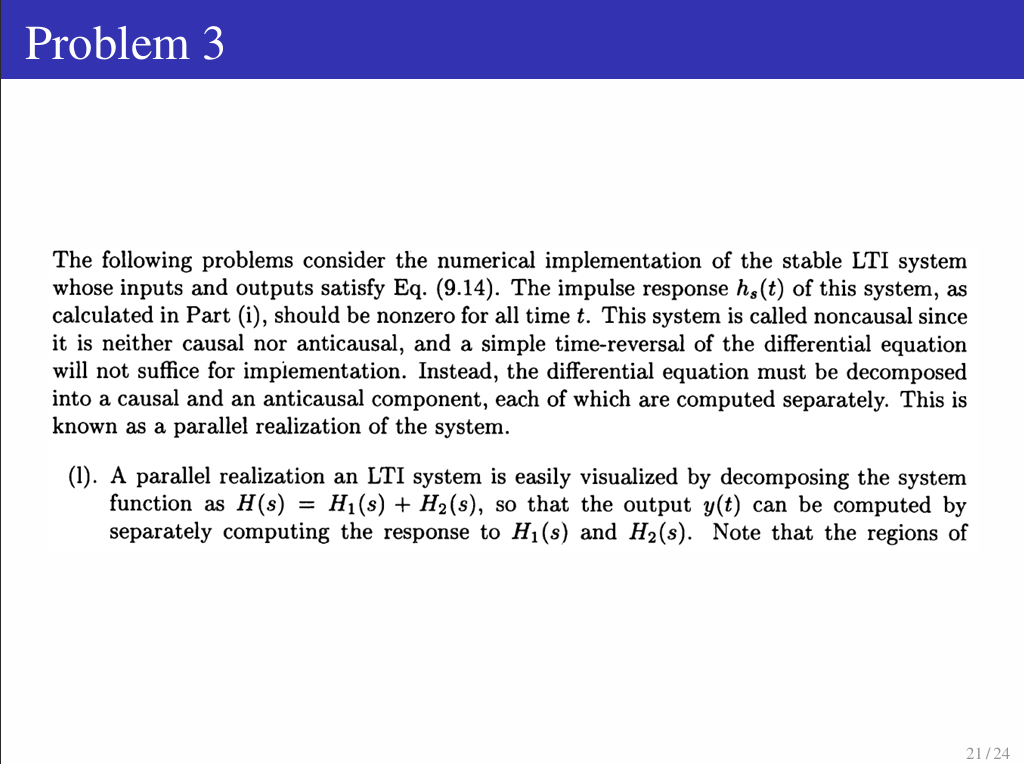
\includegraphics[width=0.9\textwidth]{figures/p36.png}
      \caption{Problem3}
  \end{minipage}%
  \begin{minipage}[b]{0.33\linewidth}
      \centering
      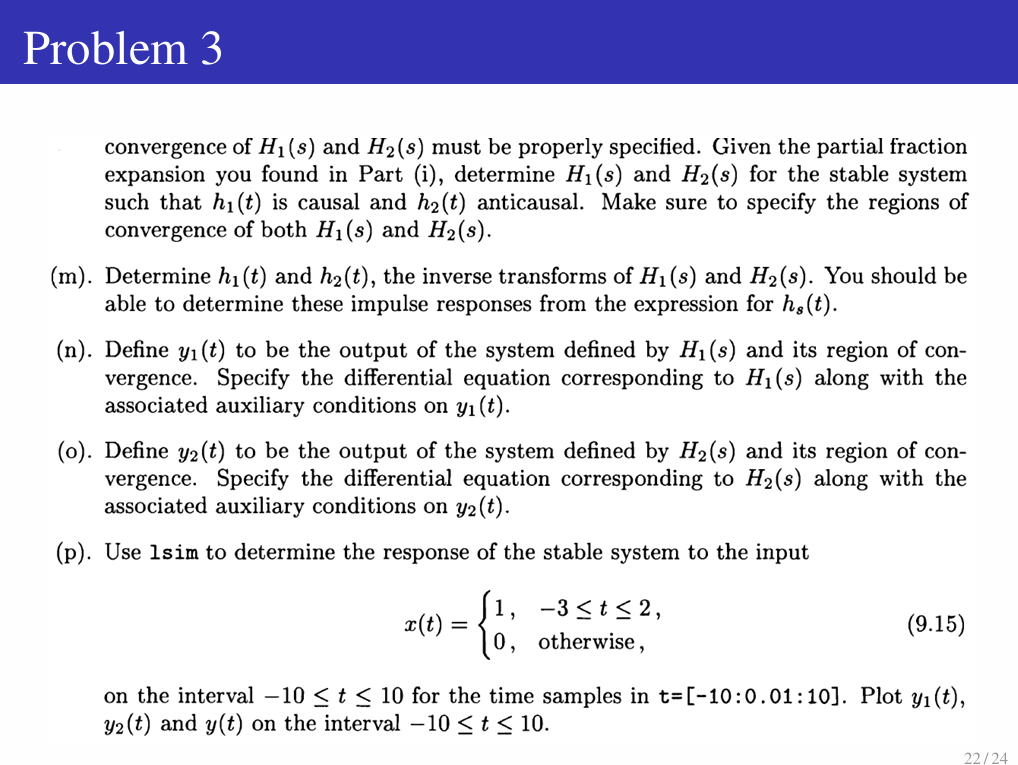
\includegraphics[width=0.9\textwidth]{figures/p37.png}
      \caption{Problem3}
  \end{minipage}
\end{figure}

\subsection{Answer}
\subsubsection{Answer h}
\[
\left( s^3 + s^2 + 24s - 26 \right) Y(s) = \left( s^2 + 7s + 21 \right) X(s)
\]
\[
H(s) = \frac{Y(s)}{X(s)} = \frac{s^2 + 7s + 21}{s^3 + s^2 + 24s - 26}
\]

\begin{enumerate}
    \item Right-sided (Causal): $\Re(s) > 1$ (excludes the imaginary axis, unstable).
    \item Two-sided: $-1 < \Re(s) < 1$ (includes the imaginary axis, stable).
    \item Left-sided (Anticausal): $\Re(s) < -1$ (excludes the imaginary axis, unstable).
\end{enumerate}
\[
\text{The system is stable only for the ROC } -1 < \Re(s) < 1, \text{ as it includes the } j\omega\text{-axis.}
\]
\begin{figure}[H]
  \centering
  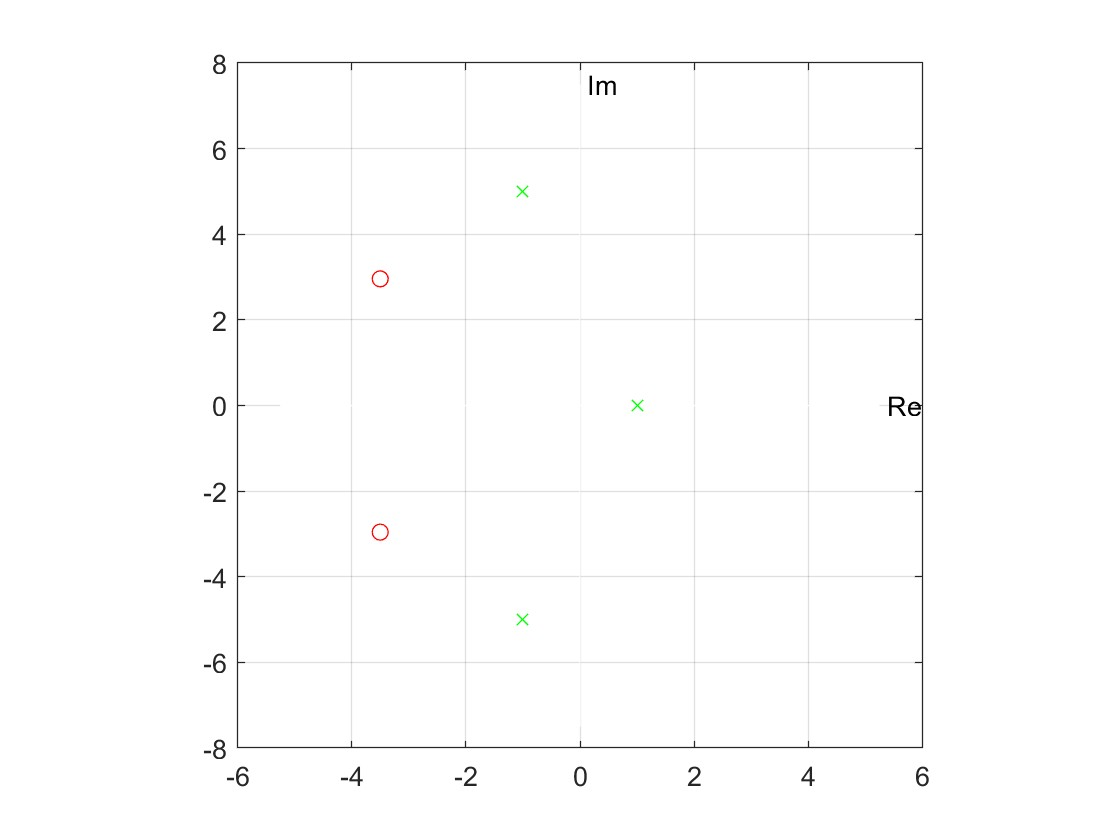
\includegraphics[width=0.35\linewidth]{figures/p3h.jpg} % 数字表示放缩比例
  \caption{Answer3h} % 图片标题
  \label{Prob1c} % 图片tag，用于交叉引用
\end{figure}
\subsubsection{Answer i}l
the values of [r,p,k] are demonstrated below
\begin{figure}[H]
  \centering
  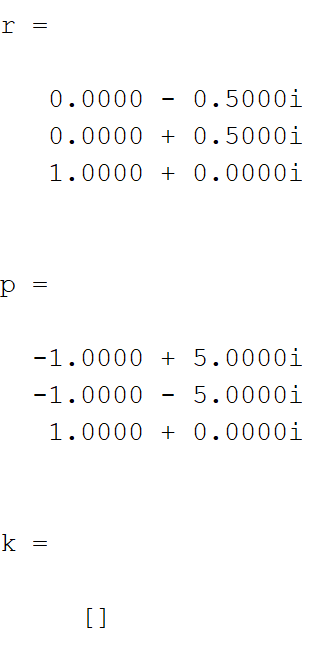
\includegraphics[width=0.3\linewidth]{figures/p3i.jpg} % 数字表示放缩比例
  \caption{Answer3i} % 图片标题
  \label{Prob1c} % 图片tag，用于交叉引用
\end{figure}
\[
H(s) = \frac{1}{s - 1} + \frac{-0.5j}{s - (-1 + 5j)} + \frac{0.5j}{s - (-1 - 5j)}
\]
\[
\begin{aligned}
  1. \, \text{ROC} : \Re(s) > 1, & \quad h(t) = \left[ e^t + e^{-t} \sin(5t) \right] u(t) \\
  2. \, \text{ROC} : \Re(s) < -1, & \quad h(t) = - \left[ e^t + e^{-t} \sin(5t) \right] u(-t) \\
  3. \, \text{ROC} : -1 < \Re(s) < 1, & \quad h(t) = - e^t u(-t) + e^{-t} \sin(5t) u(t)
\end{aligned}
\]

\subsubsection{Answer j}
\[
  case1:h(t) = \left[ e^t + e^{-t} \sin(5t) \right] u(t)
\]


The auxiliary conditions are initial rest conditions

\begin{figure}[H]
  \centering
  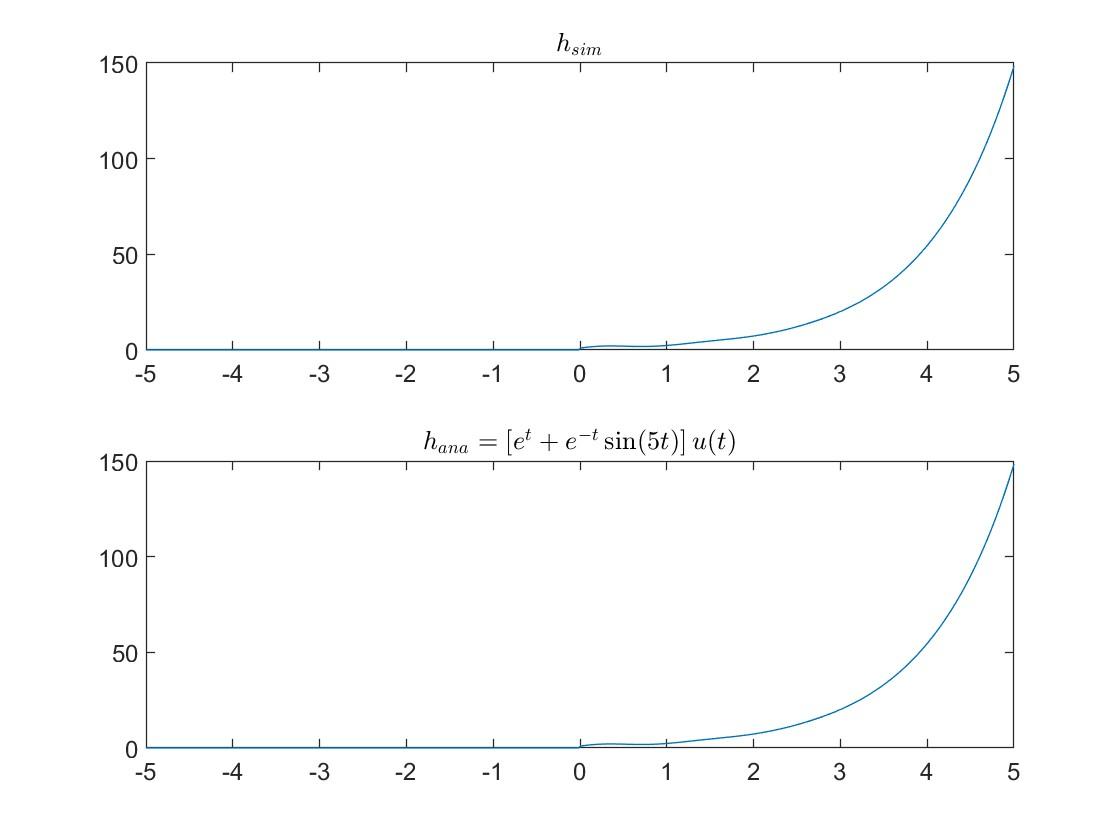
\includegraphics[width=0.5\linewidth]{figures/p3j.jpg} % 数字表示放缩比例
  \caption{Answer3j} % 图片标题
  \label{Prob1c} % 图片tag，用于交叉引用
\end{figure}

\subsubsection{Answer k}
\[
  case2:h(t) = -\left[ e^t + e^{-t} \sin(5t) \right] u(-t)
\]

The auxiliary conditions are final rest conditions

\begin{figure}[H]
  \centering
  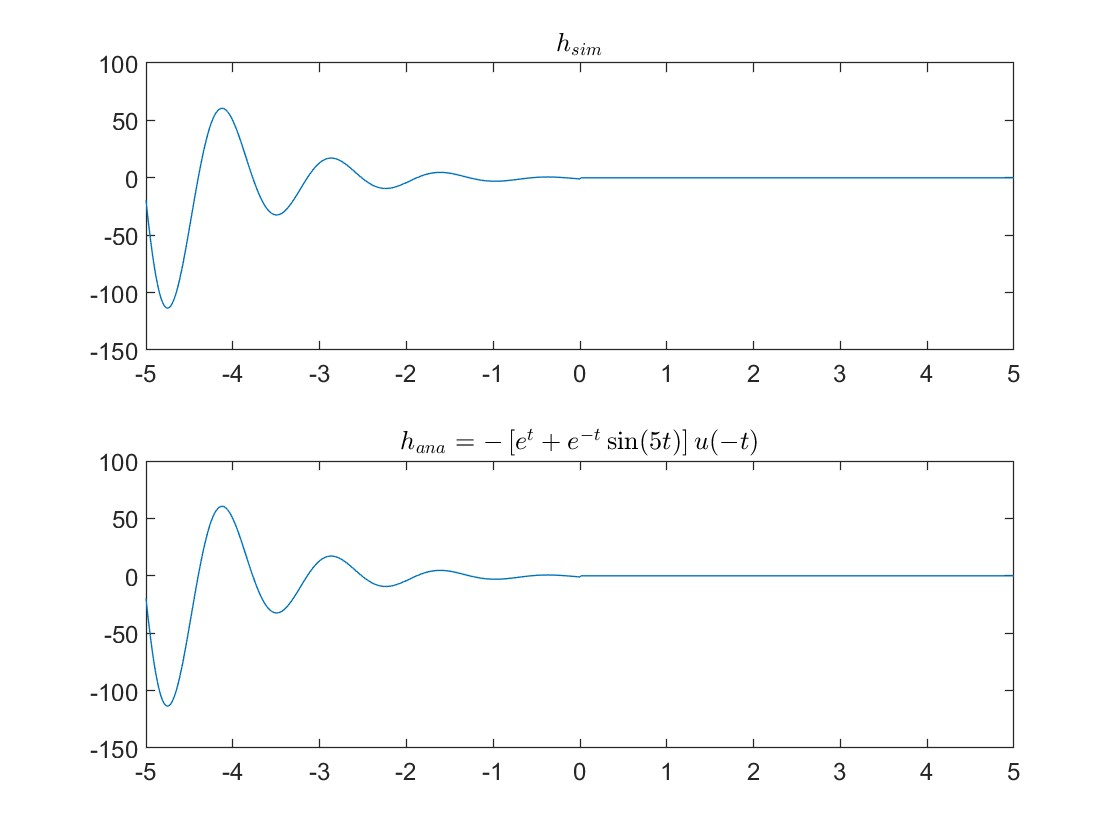
\includegraphics[width=0.5\linewidth]{figures/p3k.jpg} % 数字表示放缩比例
  \caption{Answer3k} % 图片标题
  \label{Prob1c} % 图片tag，用于交叉引用
\end{figure}

\subsubsection{Answer l}
\[
  case3: h(t) = - e^t u(-t) + e^{-t} \sin(5t) u(t)
\]

\[
H(s) = 
\underbrace{\frac{5}{(s + 1)^2 + 25}}_{H_1(s)}
+
\underbrace{\frac{1}{s - 1}}_{H_2(s)} 
\]
\[
H_1(s) = \frac{5}{(s + 1)^2 + 25} \quad \text{with ROC: } \Re(s) > -1
\]

\[
H_2(s) = \frac{1}{s - 1} \quad \text{with ROC: } \Re(s) < 1
\]

\subsubsection{Answer m}

\[
h(t) =
\underbrace{e^{-t} \sin(5t) u(t)}_{h_1(t)}
+
\underbrace{[- e^t u(-t)]}_{h_2(t)} 
\]

\subsubsection{Answer n}
\[
\frac{d^2 y(t)}{dt^2} + 2 \frac{dy(t)}{dt} + 26 y(t) = 5 x(t)
\]


The auxiliary conditions are initial rest conditions

\subsubsection{Answer o}
\[
\frac{dy(t)}{dt} - y(t) = x(t)
\]

The auxiliary conditions are final rest conditions

\subsubsection{Answer p}
\begin{figure}[H]
  \centering
  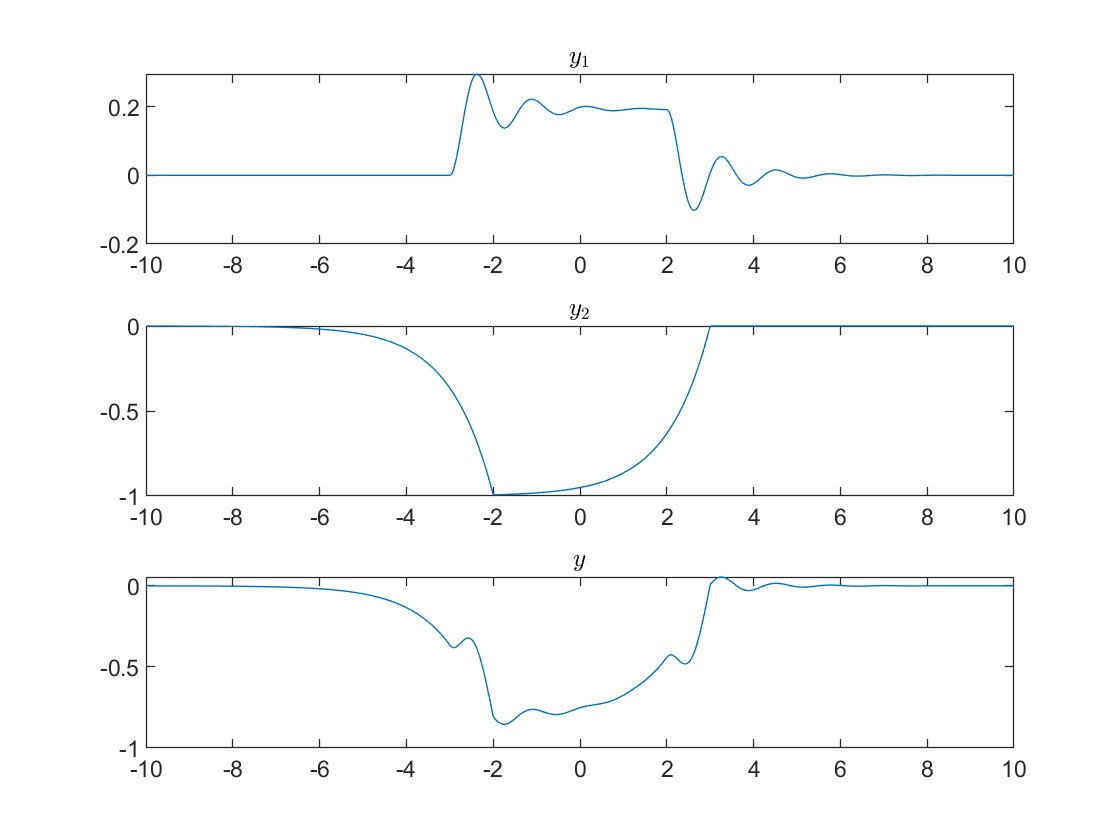
\includegraphics[width=0.5\linewidth]{figures/p3p.jpg} % 数字表示放缩比例
  \caption{Answer3p} % 图片标题
  \label{Prob1c} % 图片tag，用于交叉引用
\end{figure}
\clearpage

\section{Code}
\subsection{Code1}
\begin{lstlisting}[language=matlab, caption=Answer1a]
  clear;
  clc;

  b1 = [1 5];
  b2 = [2 5 12];
  b3 = [2 5 12];

  zs1 = roots(b1);
  zs2 = roots(b2);
  zs3 = roots(b3);

  a1 = [1 2 3];
  a2 = [1 2 10];
  a31 = [1 2 10];
  a32 = [1 2];
  a3 = conv(a31,a32);

  ps1 = roots(a1);
  ps2 = roots(a2);
  ps3 = roots(a3);

  figure
  plot(real(zs1),imag(zs1),'o');
  hold on;
  plot(real(ps1),imag(ps1),'x');
  grid;
  axis([-5 0 -2 2]);

  figure
  plot(real(zs2),imag(zs2),'o');
  hold on;
  plot(real(ps2),imag(ps2),'x');
  grid;
  axis([-2 0 -3 3]);

  figure
  plot(real(zs3),imag(zs3),'o');
  hold on;
  plot(real(ps3),imag(ps3),'x');
  grid;
  axis([-3 0 -3 3]);
\end{lstlisting}


\begin{lstlisting}[language=matlab, caption=Answer1c]
  clear;
  clc;

  b = [1 2 5];
  zs = roots(b);

  a = [1 -3];
  ps = roots(a);

  plot(real(zs),imag(zs),'o');
  hold on;
  plot(real(ps),imag(ps),'x');
  grid;
  axis([-2 4 -3 3]);
\end{lstlisting}

\clearpage
\subsection{Code2}
\begin{lstlisting}[language=matlab, caption=Answer2a]
  clear;
  clc;

  a=[1 3 2];
  b=[1 -1 0];
  dpzplot(b,a);
\end{lstlisting}

\begin{lstlisting}[language=matlab, caption=Answer2b]
  clear;
  clc;

  a=[1 3 2];
  b=[1 -1 0];
  dpzplot(b,a);
\end{lstlisting}

\begin{lstlisting}[language=matlab, caption=Answer2c]
  clear;
  clc;

  a=[1 -1.25 0.75 -0.125];
  b=[1 0.5];
  dpzplot(b,a);
\end{lstlisting}

\clearpage
\subsection{Code3}
\begin{lstlisting}[language=matlab, caption=Answer3d]
  clear;
  clc;
  
  t=-5:0.01:5;
  t_=0:0.01:5;
  
  a=[1 2];
  b=1;
  
  hs=impulse(b,a,t_);
  hs=[zeros(length(t)-length(hs),1); hs];
  
  y=exp(-2*t).*(t>=0);
  
  subplot(2,1,1);
  plot(t,hs);
  title('hs');
  
  subplot(2,1,2);
  plot(t,y);
  title('$e^{-2t}\mu (t)$','Interpreter','latex')
\end{lstlisting}

\begin{lstlisting}[language=matlab, caption=Answer3e]
  clear;
  clc;

  t=-5:0.01:5;
  t_=0:0.01:5;

  a=[-1 2];
  b=1;

  hs=impulse(b,a,t_);
  hs=[zeros(length(t)-length(hs),1);hs];
  hs=flip(hs);

  y=-exp(-2*t).*(t<=0);

  subplot(2,1,1);
  plot(t,hs);
  title('hs');

  subplot(2,1,2);
  plot(t,y);
  title('$-e^{-2t}\mu (-t)$','Interpreter','latex')
\end{lstlisting}

\begin{lstlisting}[language=matlab, caption=Answer3f]
  clear;
  clc;
  
  t=-5:0.01:5;
  t_=0:0.01:5;
  
  a=[-1 2];
  b=1;
  
  x=exp(5*t/2).*(t<=0);
  x_r=exp(-5*t/2).*(t>=0);
  
  y_sim=lsim(b,a,x_r,t);
  y_sim=flip(y_sim);
  
  y_ana = (2/9)*exp(2.5*t).*(t <= 0) - (2/9)*exp(-2*t).*(t <= 0);
  
  subplot(2,1,1);
  plot(t,y_sim);
  title('$y_{sim}$','Interpreter','latex')
  
  subplot(2,1,2);
  plot(t,y_ana);
  title('$y_{ana}=(\frac{2}{9} \cdot e^{\frac{5}{2}t}  - \frac{2}{9} \cdot e^{-2t}) \cdot u(-t) $','Interpreter','latex')
\end{lstlisting}



\begin{lstlisting}[language=matlab, caption=Answer3h]
  clear;
  clc;

  a=[1 1 24 -26];
  b=[1 7 21];
  pzplot(b,a);
\end{lstlisting}

\begin{lstlisting}[language=matlab, caption=Answer3i]
  clear;
  clc;
  
  b=[1 7 21];
  a=[1 1 24 -26];
  
  [r,p,k]=residue(b,a);
\end{lstlisting}

\begin{lstlisting}[language=matlab, caption=Answer3j]
  clear;
  clc;
  
  a = [1 1 24 -26];
  b = [1 7 21];
  t = -5:0.01:5;
  t_ = 0:0.01:5;
   
  h_ana = (exp(t)+exp(-t).*sin(5*t)).*(t>=0);
  
  h_sim = impulse(b,a,t_);
  h_sim = [zeros(500,1);h_sim];
  
  subplot(2,1,1);
  plot(t,h_sim);
  title('$h_{sim}$','Interpreter','latex')
  
  subplot(2,1,2);
  plot(t,h_ana);
  title('$h_{ana}=\left[ e^t + e^{-t} \sin(5t) \right] u(t) $','Interpreter','latex')
\end{lstlisting}

\begin{lstlisting}[language=matlab, caption=Answer3k]
  clear;
  clc;
  
  a = [-1 1 -24 -26];
  b = [1 -7 21];
  t = -5:0.01:5;
  t_ = 0:0.01:5;
  
  h_ana = -(exp(t)+exp(-t).*sin(5*t)).*(t<=0);
  
  h_sim = impulse(b,a,t_);
  h_sim = [zeros(500,1);h_sim];
  h_sim = flip(h_sim);
  
  subplot(2,1,1);
  plot(t,h_sim);
  title('$h_{sim}$','Interpreter','latex')
  
  subplot(2,1,2);
  plot(t,h_ana);
  title('$h_{ana}=-\left[e^t + e^{-t} \sin(5t) \right] u(-t) $','Interpreter','latex')
\end{lstlisting}

\begin{lstlisting}[language=matlab, caption=Answer3p]
  clear;
  clc;
  
  t=-10:0.01:10;
  
  a1=[1 2 26];
  b1=5;
  
  x=(t>=-3).*(t<=2);
  x_r=(t>=-2).*(t<=3);
  
  y1=lsim(b1,a1,x,t);
  
  a2=[-1 -1];
  b2=1;
  
  y2=lsim(b2,a2,x_r,t);
  y2=flip(y2);
  
  subplot(3,1,1);
  plot(t,y1);
  title('$y_{1}$','Interpreter','latex')
  
  subplot(3,1,2);
  plot(t,y2);
  title('$y_{2}$','Interpreter','latex')
  
  subplot(3,1,3);
  plot(t,y1+y2);
  title('$y$','Interpreter','latex')
\end{lstlisting}

\end{document}
